%% LaTeX2e class for seminar theses
%% sections/content.tex
%% 
%% Karlsruhe Institute of Technology
%% Institute for Program Structures and Data Organization
%% Chair for Software Design and Quality (SDQ)
%%
%% Dr.-Ing. Erik Burger
%% burger@kit.edu
%%
%% Version 1.0.2, 2020-05-07
\section{Foundations}
Before we go to the main sections of this seminar work, there should be introduced the main terms and concepts that are necessary for understanding and will be used during the whole work.
	\subsection{Ontology in Computer Science}
	
		\subsubsection{Ontology languages}
		The short historical survey of ontology languages approaches, based on lectures notes of course \grqq{Ontology and knowledge representation} from Prof. Boris Konev  Head of Department of Computer Science, the University of Liverpool, UK and member of the Knowledge Representation Research Group \cite{Kon10}. 
		In this sequence
			\begin{itemize}
				\item Resource Description Framework Schema: the first standard of W3C for ontologies \cite{rdfs04}, its semantic power and drawbacks
				\item Description Logic: introduction in Description Logic, EL language, its architecture and semantic
				\item Web Ontology Language: the newest standard of W3L based on Description Logic \cite{owl04}
			\end{itemize}
		\subsubsection{Expediency and reasons for using of Ontologies}
		Here is discussed, when and where the onologies should be used and when it is superfluous
		\subsubsection{Examples of Ontologies}
		Here come the examples of ontologies in medicine, then in Meta-research and SE.
		
	\subsection{Meta-research}
		\subsubsection{Motivation}
		A statement \flqq{Science is one of the main driver of human progress}\frqq is indisputable and proved by growing number of published papers and publishing authors\cite{Ioa14}. Naturally people face the problems such as data sharing, replications of experiments, its ownership and many others. Moreover, the research practices suffer from lack of systematization and inefficiency. For example, according to \cite{Mac14}  85\% of resources in biomedical research are wasted because of above-called reasons. Therefore, there exists the urgent need of Meta-research, which aims to include the evaluation of diverse researches with succeeding suggestions of improvement for research practices.    
		
		 
		\subsubsection{Ares of Meta-research}
		Discussing the existing problems about contemporary research the logical question arises: is it possible to provide a map of ongoing efforts in the field Meta-research and connect the multiple already made, but still fragmented attempts across science. These goals were set by J. Ioannidis in its work \flqq{Meta-research: Evaluation and Improvement of Research Methods and practices}\frqq \cite{Ioa15}. \newline
		His suggestions can be summed up in the following categorization. There are five major areas of interests in meta-research: methods, reporting, reproducibility, evaluation and incentives. Each of them was not only explicitly defined and with examples illustrated, but also for each area the existing initiatives were found. These mentioned features of the work can be summarized as following categorizations:
		\label{sec:AreasOfMetaresearch:cat}  
		\begin{enumerate}
			\item{\textbf{Methods}:} practices for performing research  (\textbf{e.g.} study design, methods, statistics). With \textbf{specific interests} in biases and questionable practices in conducting
			research, methods to reduce such biases, metaanalysis. Existing \textbf{Initiatives} such as Cochrane Collaboration for systematic reviews of health care or Campbell Collaboration for the same ones but in social science.
			   
			\item{\textbf{Reporting}:} publications of standards and study registrations  (\textbf{e.g.} study registration, information to patients, public and policy-makers). With \textbf{specific interests} in biases and questionable practices in reporting, explaining, disseminating and popularizing research. Existing \textbf{Initiatives} such as ClinicalTrials.gov for clinical trials registrations or EQUATOR network for reporting standards for research.
			
			\item\textbf{{Reproducibility}:} methods for verifying research (\textbf{e.g.} sharing data and methods, replicability). With \textbf{specific interests} in overcoming of obstacles to sharing data, methods and replications. Existing \textbf{Initiatives} such as YODA for sharing data in clinical research or BITSS for transparency in social science. 
			
			\item{\textbf{Evaluation}:} approvements for scientific quality (\textbf{e.g.} pre- and postpublication peer reviews, research funding criteria). With \textbf{specific interests} in  effectiveness, costs, and benefits of old and new approaches to peer review. Existing \textbf{Initiatives} such as Peer Review Congress for evidence on peer review or ArXiv for preprinting articles. 
			 
			\item{\textbf{Incentives}:} rewards and penalties for research (\textbf{e.g.} promotion criteria, penalties in research evaluation). With \textbf{specific interests} in Accuracy, effectiveness and benefits of old and new approaches to ranking and evaluating the performance. Existing \textbf{Initiatives} such as REWARD for reducing waste and rewarding diligence in research or AAAS for science policy.
		\end{enumerate}
		 Certainly, it has to be said that this is an \flqq{nonexhaustive list}\frqq. Also, it is worth of remarking that neither in this paper nor in referenced and citating papers the initiatives in SE-Meta-Research are considered. Therefore, strictly based on definitions and comparing of initiatives in other fields, the mentioned in this work approaches in Software Engineering will be categorized, if it is possible and if not, discussed limitations of such classification. 
		
		

\section{Ontology in Software-Engineering-Meta-Research}
This section aims to show different types of ontologies, which are used by scientists for Meta-research in Software Engineering, and also to compare them.  \newline
 Firstly, in order to show all this diversity, the Biolchini's\cite{Bio07} classification of empirical studies in SE has been chosen. It shows \flqq{the concepts of Primary and Secondary Studies on Software Engineering at a high level}\frqq\cite[p. 1]{Gar08}. According to this classification any experimental study comprises two types of investigations: Primary and Secondary\cite[p. 134]{Bio07}. Primary studies are used for evaluation of the researcher's hypothesis and represented above all by Controlled Experiments. In contrast, Secondary studies serve for comparisons between individual investigations to generalize the results and are represented by systematic reviews. \newline
 Secondly, in order to make the introduced ontologies comparable, the template  \flqq{Problem, Objectives, Suggested method and Future works}\frqq that was used by me during the reading of papers, will be applied. Although this segmentation cannot transfer the whole information contained in papers, it should be sufficient for the set intentions.
    
 
	\subsection{Ontology to support systematic reviews in Software Engineering}  
	Before we go to systematic reviews, let me introduce Evidence-based Software Engineering(EBSE), whose main instrument they are. EBSE was evolved by Kitchenham\cite{Kit04}. The author supposes that SE might benefit from an evidence-based methods, as it was done in medicine with appearance of Evidence-based Medicine(EBM). The goal of EBSE is \flqq{to provide the means by which current best evidence from research can be integrated with practical experience and human values in the decision making process regarding the development and maintenance of software}\frqq \cite[p. 2]{Kit04}. In other words, what SE practice works,  when, where and which tools and standards are needed for that. This all can and should be proven by experiments using Systematic reviews(SRs), where SRs are \flqq{form of secondary study that uses a well-defined methodology to identify, analyse and interpret all available evidence related to a specific research question in a way that is unbiased and (to a degree) repeatable. }\frqq [Link to guidelines kitchenham] or simplified a tool to obtain accurate knowledge by analyzing the primary studies to eliminate possible biases. \newline
	
	Having so detailed introduction of origin SRs, Biolchini has set a \textbf{Problem}: produce knowledge that can be based on scientific methodology. Besides, according to his work this problem implies the following \textbf{Objectives}:
		\begin{itemize}
			\item Discussing the significance of experimental studies, particularly SRs and their use in supporting software processes
			\item Present a template designed to support systematic reviews in SE
			\item Introduce development of ontologies to describe knowledge regarding such experimental studies
		\end{itemize}
	\label{sec:OntSRinSE:guidelines}    
	So as to fulfill the determined objectives, the author introduces, firstly, a template for systematic review protocol(\autoref{fig:srprotocol}) that was created based corresponding Guidelines\cite{Kit07} and own experience. It is worth to notice the later relevant parts of them, such as Problem (SR target, describing the research context), Intervention(observation target in SR), control(initial data already possessed by researcher), outcome measure (metrics to measure effects), experimental design(which statistical analysis method will be applied on the collected data).
	\begin{figure}
		\centering
		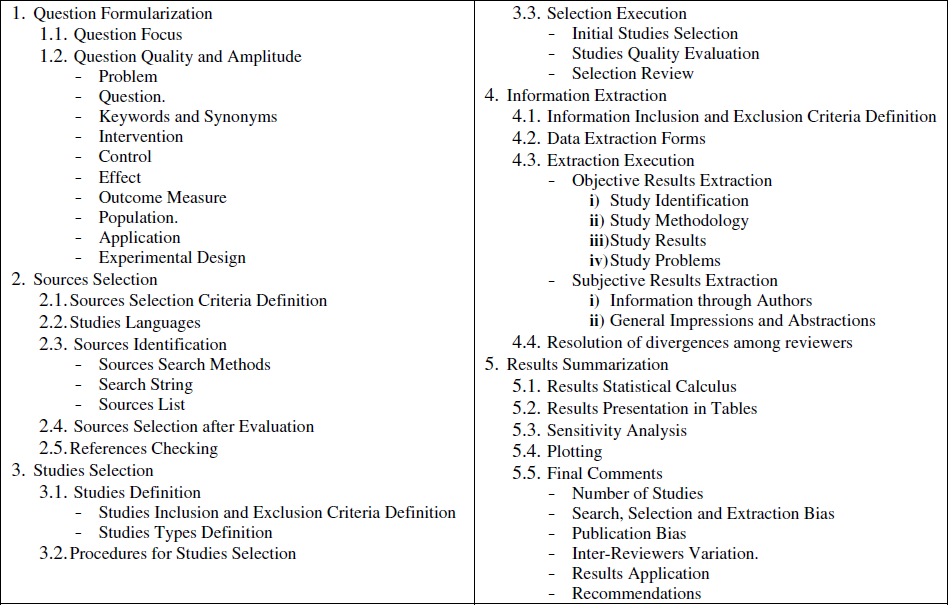
\includegraphics[width=15cm]{images/SRreviewprotocol.PNG}
		\caption{Systematic review protocol template\cite[p. 142]{Bio07}}
		\label{fig:srprotocol}
	\end{figure}
	 \newline
	
	Secondly, the author \textbf{suggest} \flqq{Scientific research ontology}\frqq that is organized in level-structure (entities of levels can be seen as concepts) and the levels posses taxonomic and meronomyc hierarchies (can be seen as roles), namely is\_a and has relations. The following paragraph summarizes and analyzes the main components and features of the suggested ontology level by level with pertaining relations between them.
		\begin{itemize}
			\item[\textbf{Level 0:}]  Different knowledge of domains that are involved in the conduction of SRs in SE, represented by \textit{Experimental Method}, \textit{Primary Research} and \textit{Research Synthesis} 
		\end{itemize}
	For the further discussion the domain \textit{Primary Research} is selected, but the analog statements and conclusions can be derived and provided by remaining ones.
		\begin{itemize}
			\item[\textbf{Level 1:}] The conceptual entity, represented by \textit{Primary Study Element} is the highest level of hypernym of the \textit{Primary Research} and subsumes the concepts in the lower levels of hierarchy.
			\item[\textbf{Level 2:}] The main concepts, represented by \textit{Structure of Study} and \textit{Quality of Study} 
			\item[\textbf{Level 3:}] The subcategories of one of the main concept Structure of study, represented by \textit{Problem, Hypothesis, Intervention, Control, Measurement, Outcome} and \textit{Unit of Study}
			\item[\textbf{Level 4:}] The entities of the subcategory \textit{Outcome} that is demonstrating the ontological hybridism, having not only taxonomic relations, represented by \textit{Target Outcome} and \textit{Surrogate Outcome}, but also meronymic relations, represented by \textit{Endpoint, Incidence, Prevalence, Effect Modification} and \textit{Effect Modifier} 
		\end{itemize}
	  As we can observe, the above described part of the ontology \textbf{results} in an object that directly linked with Systematic review protocol template. The full ontology concepts an roles can ve read in the paper, but the given example in depth of levels depicts the power comprehensive cover of SR needs. \newline
	  
	  Though the presented ontology was at the moment of publication only in development, it can esteemed as robust for entire diversity of SRs in different types of Studies. Nevertheless, the  author points on possible \textbf{future works}, which are mainly related to merging of the presented Scientific Research Ontology with Software Engineering Ontology and successive integrating them into eSEE (experimental Software Engineering Environment). Moreover, this could lead towards a wider Experimental Software Engineering Ontology that theoretically will combine all received evidence-based knowledge in Software Engineering.  
	 
	
	\subsection{Ontologies for Controlled Experiments on Software Engineering}
	In contrast to the previous subsection, this one is about a part of Primary Studies, where one of the main subjects are Controlled Experiments. They serve Experimental Software Engineering as an instrument to build a body of knowledge for diverse and exceeding software practices to support making successful decision in SE. \newline
	
	Obviously, there exist many problems in this field and one of them is trying to be solved by R. E. Garcia\cite{Gar08}. This \textbf{Problem} is sharing of knowledge among research groups. It requires replication of Controlled Experiments. The generated Knowledge during these experiments is registered in so-called Lab Packages (procedures, the results and conclusions). However, researchers face difficulties reviewing the lab packages and suffer from the lack of standardization, what leads to obstacles in sharing knowledge among research groups. \newline
	
	According to the problem there were set the following \textbf{Objectives:}
		\begin{itemize}
			\item Explore ontologies to support knowledge transfer,
			helping to elucidate the associated concepts of controlled
			experiments and their relationships.
			\item Present an Ontology to experimental studies, named EXPEROntology - tool
			for knowledge transfer, assisting researchers, reviewers,
			and meta-analysts in designing, conducting, and evaluating
			controlled experiments.
			\item Validate the ontology, whilst instantiating it to a controlled experiment.
		\end{itemize}
	  
	Before we come to the suggested ontology, it is noteworthy to talk about the main object of the current research, in particular five Controlled Experiments phases and its components\cite{Woh00}: 
	\begin{enumerate}
		\item Definition: hypotheses and experiment goals
		\item Planning: execution plan and environment; subjects and their profiles; dependent and independent variables; validity 
		\item Operation: preparation, execution, data validation
		\item Analysis: analysis of collected data
		\item Packaging : artifacts, procedures, results into Lab Packages (is recommended executing parallel with each phase)
	\end{enumerate}    
	Some above named components show up in the \textbf{suggested} ontology, which can be seen on \autoref{fig:ontforce} and has the following ordered workflow, consisting as usual of concepts and roles (relations) between them: 
	\begin{enumerate}
		\item \textit{Lab Package} from \textit{Original Experiment} (created by \textit{Designer}) is used for \textit{Replication} (by \textit{Replicator}) and generation of a new \textit{Lab Package}.
		\item \textit{Designer} and \textit{Replicator} have \textit{Experimenter Profile}: negative influence attests a lack of experience, positive - high experience
		\item \textit{Original Experiment} and \textit{Replication} evaluated regarding to \textit{Validity} with four types: conclusion (relationship between the treatment and outcome), internal (relationship between the factors and the outcome), construct (relation theory and observation and external(generalization).	
	\end{enumerate}

	\begin{figure}
		\centering
		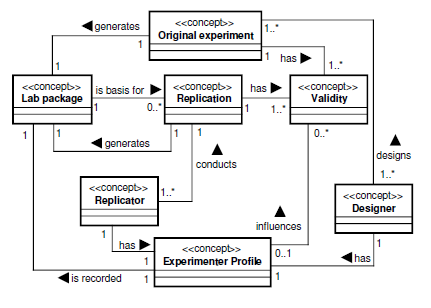
\includegraphics[width=10cm]{images/OntforCE.PNG}
		\caption{Ontology for Controlled Experiment\cite[p. 3]{Gar08}}
		\label{fig:ontforce}
	\end{figure}
	\begin{figure}
		\centering
		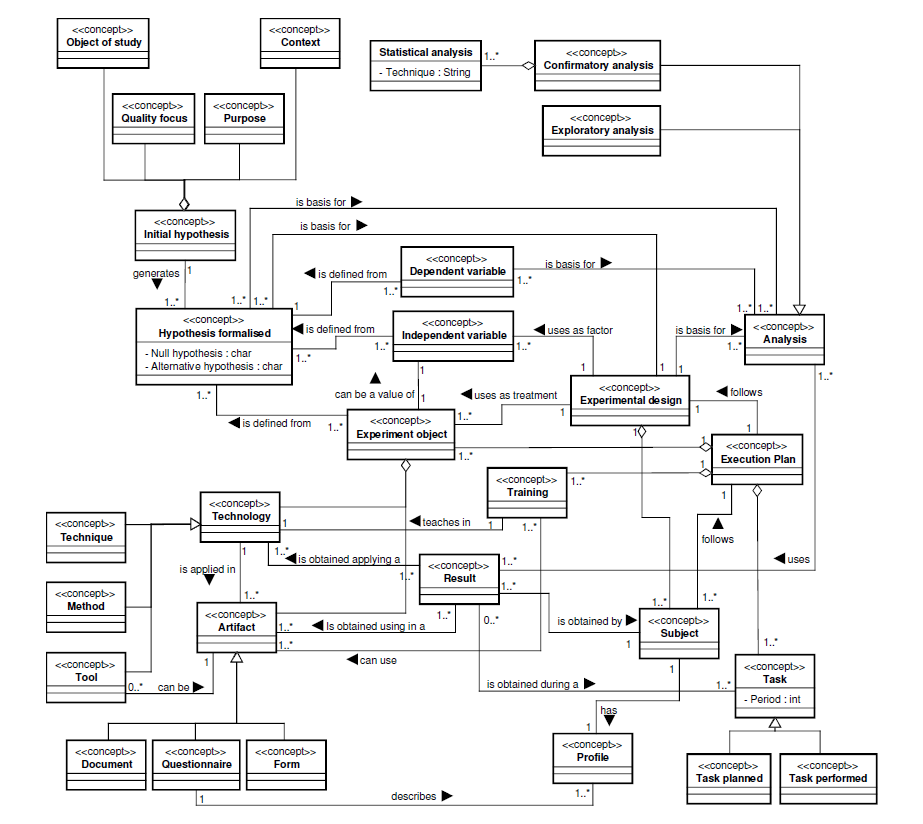
\includegraphics[width=18cm]{images/OntforLP.PNG}
		\caption{Ontology for Lab Packages\cite[p. 4]{Gar08}}
		\label{fig:ontforlp}
	\end{figure}
	But so superficial-designed is apparently not be able to sophisticate all needs of researchers. Therefore, Garcia goes deeper and refine the above described ontology,  presenting the EXPEROntology for Lab Package that can be observed on \autoref{fig:ontforlp}. Besides, four years later the author publishes the guidelines for this ontology\cite{Gar11}, extending the earlier work and providing more circumstantial description of that. Let us focus below on the main structures and features of the presented ontology, corresponding to it workflow and how it refers to earlier set up phases of Controlled Experiments:
	\begin{enumerate}
		\item Definition: establishing of \textit{Initial hypothesis}, composed by \textit{Object of study, Purpose, Quality focus} in a specific \textit{Context}.
		\item Planning: generating \textit{Hypothesis formalized} from Definition phase. Experimenter defines \textit{Dependent, Independent Variables} and \textit{Experimental Object} that contains \textit{Technology} and \textit{Artifacts} to be used in controlled experiment. Furthermore, in this phase the \textit{Experimental design} is created and refined by \textit{Subject} and its \textit{Profile}.
		\item Operation: elaborating \textit{Execution plan}, which is obtained by \textit{Task}s 
		\item Analysis: gathering \textit{Result}s from Operation phase are to be used in \textit{Analysis} of different types, such as \textit{Confirmatory}(testing \textit{Hypothesis formalized}) or \textit{Exploratory}(investigating new relationships)   
	\end{enumerate}
	Since it is desired to make all these concepts working, we are missing the connection axioms for the entire ontology. It is enough to define four predicates:
	\begin{enumerate}
		\item
		\begin{align*}
		 Design(subject, SetOfTreatment)
		\end{align*} 
		\item 
		\begin{align*}
			Factor(f1,...,fn) \\
			 \forall f \in Factor,\ \exists Treatment(f) = {v_1,...,v_n}, n \ge 2 \\
			dom(Treatment) = Artifact \cup Technology \\
			SetOfTreatment = (vf_1,...,vf_n)|\forall f, vf_n \in Treatment(fn)
		\end{align*}
		\item 
		\begin{align*}
			\forall subject, SetOfTreatment \\
			Execution(subject, SetOfTreatement) \rightarrow Task(ta_1) \land...\land Task(ta_n)
		\end{align*}
		\item 
		\begin{align*}
			Task(ta_n) \rightarrow Training(subject,t_r,a,p) \lor Applying(subject,t_e,a,p)
		\end{align*}
		
	\end{enumerate}
	The last, but not least is validating of presented ontology by obtaining the \textbf{Results} on existing data. Thus, in order to illustrate the power of the suggested ontology, it has been chosen an experiment that was originally conducted by Basili and Selby\cite{Bas87}. The objective of the study was \flqq{compare three state-of-the-practice software testing techniques: a) code reading by stepwise abstraction, b) functional testing using equivalence partitioning and boundary value analysis, and c) structural testing using 100 percent statement coverage criteria.}\frqq\cite[abstract]{Bas87}. So, the Experimental Design of the study: 32 Subjects were divided in 3 groups(advanced, intermediate and junior) and  each of them applied 3 software testing techniques(code reading, functional testing and structural testing) on 3 different pieces of software(text processor, numeric abstract data type and database maintainer). According to this description the EXPEROntology was instantiated as following(for instance only for one subject S1).
	\begin{enumerate}
		\item \begin{align*}
			Design(S1, Advanced, Code\ Reading, P3) \\
			Design(S1, Advanced, Functional\ Testing, P2) \\
			Design(S1, Advanced, Structural\ Testing, P1) \\
		\end{align*}
		\item \begin{align*}
			Factor = (Expertise, Technique, Program) \\
			for\ Expertise, Treatment = \{Advanced, Intermediate, Junior\} \\
			for\ Technique, Treatment = \{Code\ Reading, Functional\ Testing, Structural Testing\} \\
			for\ Program, Treatment = \{P1,P2,P3\} \\
			SetOfTreatment = {(Advanced, Code\ Reading, P3)}
		\end{align*}
		\item and 4.  
		\begin{align*}
			Execution() \rightarrow  \\
			Training(S1, \{Code\ Reading\ \lor Functional\ Testing \lor  Structural\ Testing\}, --, --) \land ... \\
			Applying(S1,\{Code\ Reading\ \lor Functional\ Testing \lor  Structural\ Testing\}, P3, --) \land ... \\
		\end{align*}
	\end{enumerate}
  
	 After the instantiating of the ontology, we can observe that all pieces of information given in the conducted study can be encapsulated and saved in EXPEROntology without loosing any information.
	 
	 Besides, we can observe the missing values on the predicate: Training - artifact and period of training, Applying - period for the application. After looking in the study we can see that it does not bring them indeed. It allows us to make one more important conclusion \flqq{the ontology can also be used as a mechanism to improve the obtained data set from the Lab Package}\frqq\cite[p. 6]{Gar08}. 
	 
	 Also, the authors intend in \textbf{Future works} compbine the presented EXPEROntology with OntoTest. By merging these two ontology it will be possible to create an whole architecture that \flqq{supports the development of environments/tools to automate, software testing activities and related experimental studies}\frqq\cite[p.6]{Gar08}
	 \newline
	 
	 We have just looked at the ontology for the controlled experiments. However, there exists another work from alternative perspective, which was suggested by H. Siy and Y. Wu\cite{SiyWu12}. Although they had the similar \textbf{Objectives}:
	  \begin{itemize}
	 	\item Present an ontology for analyzing empirical studies of SE, in particular the design of software engineering experiment
	 	\item Encapsulate the experience experts by means of an ontology for experimental designs using Protege OWL
	 \end{itemize}
	they are aware of the \textbf{Problem} wider in enterprise way, namely a bad designed experiment can increase the cost and risk of invalid results. And the solving this problem includes not only the fundamental knowledge of the mechanisms, methods and tools,
	thus improving our understanding of which one works best under what situation, but also the way software engineers work, think and interact with each other.
	
	So as to solve this problem, the author \textbf{suggest} the following ontology concept. First of all, the main concepts and their roles(\autoref{fig:ontwu} are presented: 
	\begin{itemize}
		\item{\textit{Treatment}} Software Engineering Technique/Method/Process being studied
		\item{\textit{Subject}} Person, Developer/Student participated on experiment
		\item{\textit{Object}} Entity, Program/Model
		\item{\textit{Assignment}} Relation between all of them; in an assignmentInstance: a subjectInstance is assigned to apply a treatmentInstance in an objectInstance. 
	\end{itemize}
	\begin{figure}
		\centering
		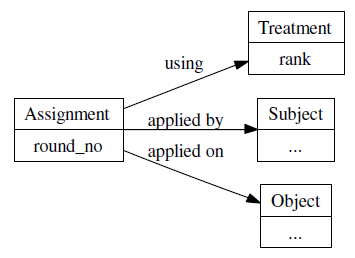
\includegraphics[width=5cm]{images/OntWu.PNG}
		\caption{Ontology fragment depicting the concepts involved in the design of experiments\cite[p. 13]{SiyWu12}}
		\label{fig:ontwu}
	\end{figure} 
	Secondly, in order to bring all these concepts working, the connection axioms are set. In sum, we get four necessary constraints and the purposes they fulfill:
	\begin{enumerate}
		\item No \textit{Subject} can be assigned a \textit{Treatment} that is less sophisticated than the other ones he was already assigned to. What for: subject assigned to one treatment may use the knowledge and experience
		gained from that treatment.
		\item No \textit{Treatment} was applied by only one \textit{Subject}. What for: experiment subjects have varying backgrounds and abilities, what implies different results. If only one subject is related, then it is not scientifically meaningful.
		\item \textit{Subject} is assigned to several \textit{Treatments}. What for: assess the variability introduced by that subject
		\item An \textit{Object} is treated by several \textit{Subjects}. What for: provide a way to untangle subject performance from object complexity
	\end{enumerate}
	
	Finally, the created ontology concept was evaluated on experiments on software inspections\cite{Bas99}. Aligning to presented concepts the concrete values i. e. \textit{Treatment} - reading technique, \textit{Subject} - reviewer, \textit{Object} - software requirements document. The \textbf{Results} were \flqq{encouraging}\frqq\cite[p. 15]{SiyWu12}. The author states no it was not found any validation after the applying all constraints. Moreover, if the ontology was fed by  invalid assignments, it was possible to observe inconsistencies as expected.
	
	It remains to be said that the authors consider the \textbf{Future} of their presented ontology and the preliminary results that it has shown as a step towards organizing and accommodating such a ontology, which can also support other Software Engineering knowledge domains(not only the systematic review process).  \newline
	
	
	To sum up, we could observe in this section four ontologies that were introduced by three different groups of researchers. Although the scientists had set different objectives and problems that they tried to solve, here can be discussed similarities of suggested in this sections ontologies. Firstly, it is remarkable that all researchers point on the advantages and opportunities which the adoption of ontologies give them in realization of their intentions. In the researcher's opinion, an ontology is the best tool to accumulate any experience or knowledge(especially, from experiments), formalize them for later representing, sharing and transferring. Nevertheless, ontology is not a silver bullet, because of apparent drawbacks. It cannot depict preciously all objects of the real world and relations between them. An ontology is still restricted by the first-order logic. But sometimes it can be enough to get desired results. Secondly, even though only Biolchini et al.\cite{Bio07} intended to work directly on the supporting of systematic reviews, the other presented ontology also pertain to them e. g. Garcia et.al.\cite{Gar08} evaluated their ontology on experiments with V\&V techniques\cite{Bas87} and H. Siy and Y. Wu \cite{SiyWu12} on experiments with software inspections\cite{Bas99}. This congeniality shows us, how important are systematic reviews and thereby EBSE in modern Software Engineering.\newline
	To the very end, let us discuss the differences between the presented ontologies. First of all, according to the categorization in \autoref{sec:AreasOfMetaresearch:cat}, the Biolchini et. al. for supporting systematic reviews\cite{Bio07} must definitely belong to the area Methods as by analogy provided initiative Cochrane Collabaration for Systematic reviews of health care; Garcia et. al. two ontologies\cite{Gar08}\cite{Gar11} exactly match the category Reproducibility, since their main objective to support replication of the SE studies; the last one by H. Siy and Y. Wu\cite{SiyWu12} might belong to as Reproducibity as Methods because of similarities with three presented before. Finally, we could observe that the modeling of each presented ontology was done by using of different ontology languages or at least different kinds of the same language what can also lead to the barriers by applying of the presented ontologies and making them standards in the research field.
	  	 
\section{Ontology-based systems in scientific search}
During the searching and reading of the suggested and found by reference-based search papers the two facts appeared in sight: Ontologies are used in contemporary search engines and the the scientific world is using ontologies successfully for a big amount of tasks. Therefore, based on database search (because this was not the original accent of the suggested literature list) the papers about Ontology-based systems in scientific search were found and will be analyzed further in this section.
		\subsection{Semantic Web}
		Every discussion about ontologies is incomplete, if the concept of Semantic web is omitted. Therefore, in this subsection the Semantic Web is presented and compared with a traditional Web (WWW).
		
		The first definition of Semantic Web was coined by T. Berners-Lee: \flqq{The Semantic Web is an extension of the current web in which information is given well-defined meaning, better enabling computers and people to work in cooperation”}\frqq\cite{Ber01}. But what are the purposes that we are not be able to use the traditional Web and urgent need the Semantic one? 
		
		Firstly, we are all aware of constant growing of our Web, namely the information in it. Thus, indexing and retrieving of information becomes an unbearable task if we do it manually or semi-automatically as it happens in the current Web. Secondly, the current Web that we have is a Web of HTML-documents (or other formats), which means only human can really understand information and referring to this relations in a document. The Semantic Web should become the Web of meaning and thereby understandable not only by humans, but also by machines. Thirdly, every language has uncountable amount of synonyms wit the same meaning, but different word representation. Besides, the current Web is getting multi-lingual. As in example: \flqq{English shopping website would use the word price to refer to an items price, while a Dutch website would use the word prijs, a French website would use the word prix...}\frqq \cite[p. 40 ]{Raj14} the same information differ in other languages and thus different for the machines. And finally, to summarize the current paragraphs, the main purposes of the Semantic Web were introduced by W3C that states \flqq{The Semantic Web is about two things. It is about common formats for interchange of data, where on the original Web we only had interchange of documents. Also it is about language for recording how the data relates to real world objects. That allows a person, or a machine, to start off in one database, and then move through an unending set of databases which are connected not by wires but by being about the same thing}\frqq\cite{w3c01}.
		
		
		\subsection{Semantic Search Engine}
		The main requirement for the Semantic Web is a search engine for the proper interpretations of the user's search intentions, ability to detect the relations between found results and pretension of them with respect to relevance.
		
		Before we go to the semantic search engine, the basic one should be surveyed. Compressed information about the traditional search engine architecture is retold further based on description in \cite{Gup12}. Before the real search query begins, the crawler indexes the already available information in the background, by  storing, marking and organizing the fetched from WWW data. It allows the search engine to collect and output data with respect to the highest page rank, when the real search query is given.
		
		Knowing the main steps of the basic search engine we are now able to see the main feature of the Semantic search engine. The thing that distinguishes the semantic search engine and brings it to the next level is using ontologies. In the following paragraph one variation of the Semantic search engine based on ontology is presented based on description of Fang. et al. \cite{Fang05}, which makes easier the discussing features and opportunities of using ontologies in semantic search.
		        
		The basic search engine suffers from a \textbf{Problem} that it searches the web documents based on keywords, but should base on their content. Therefor, there were set the \textbf{Objectives}: use ontologies as knowledge representation domain, use OWL DL to represent them and finally, employ them in search engine; create a preliminary implementation of a framework and test it. 
		
		Getting rid of particular details and summing up the algorithm, the \textbf{suggested} method has the following steps(after the input of a query):
			\begin{enumerate}
				\item Parse the keywords in the query, which relate to concepts in ontology and forward it to the Reasoner
				\item Reasoner returns RDF triples as input to the next step
				\item Retrieve the referring to these concepts documents based on extended Term-Document Matrix(TDM), where the extended TDM is constructed before, with the three steps: Calculating the basic TDM(like in a basic search engine), defining the relevance between ontologies and documents and calculating the extended TDM based on the previous step. This allow the extended TDM depicting the connections between concepts in the domain ontologies.
				\item Sort the retrieved documents by relevance and output them to the user.   
			\end{enumerate}
		
		This constriction of the semantic search engine \textbf{results} in the improving of the main parameter for the search query, namely precision and recall that can be observed on \autoref{fig:SearchEnginePR}. To be remarked, the experiment is evaluated on one topic(with corresponding ontology) in  3600 manually classified documents for three topics. Of course, it is one of the first approaches and authors' \textbf{future} works are going to optimize the relevance levels.
		\begin{figure}
			\centering
			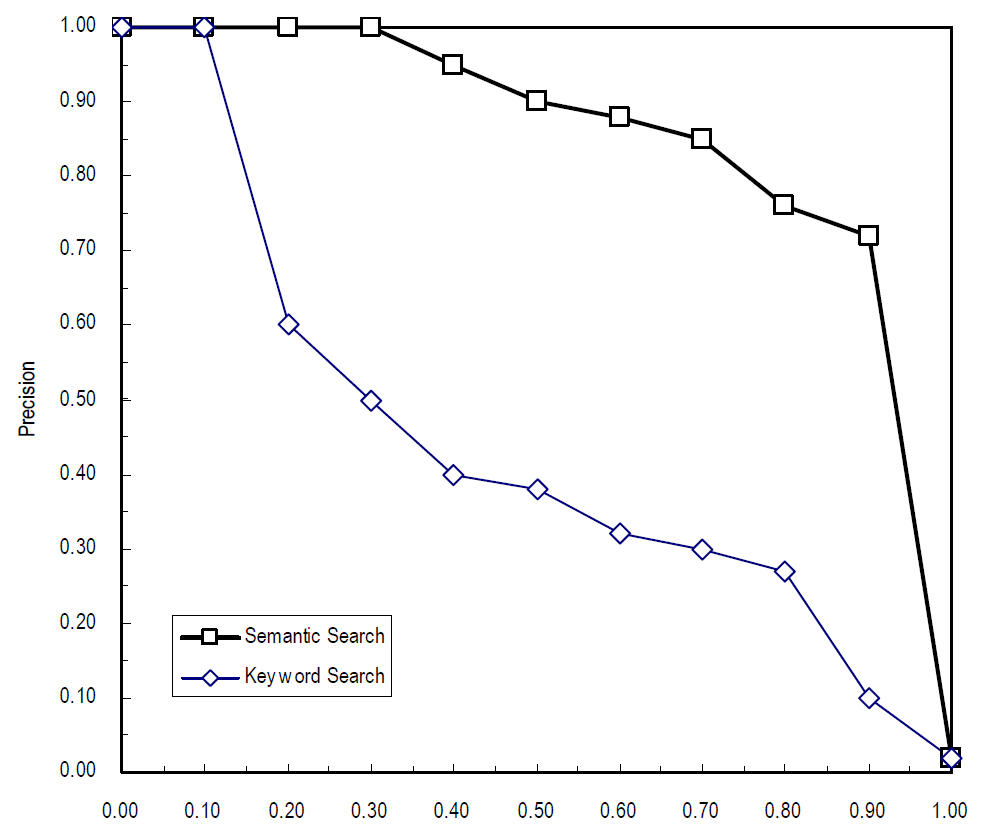
\includegraphics[width=10cm]{images/SearchEnginePR.PNG}
			\caption{Precision-recall graph comparison of semantic and keyword search\cite[p. 1918]{Fang05}}
			\label{fig:SearchEnginePR}
		\end{figure}
		To conclude the main differences between basic search engine and semantic search engine based on ontologies\cite[p.653]{Gup12}
			\begin{itemize}
				\item Query in basic search engine takes less time, but the  Result of a query in semantic search engine is much more relevant
				\item Basic search engine crawler uses all domains based o keywords. The semantic one considers the logical meaning instead. 
				\item Basic search engine construction costs in implementation and time are less, whereby the semantic one reduces costs of searching for an user   
			\end{itemize} 
		\subsection{Examples}
		As it was said in the previous subsection section the main feature of the semantic search engine is using of ontologies. But what of them should be used adopted and what left out. In the next section there will be introduced all scientific search ontologies \flqq{palette}\frqq and in the sections after that it is discussed what requirement they should fulfill how they can interact and can be used together.
		
		\subsubsection{Scientific ontologies}
		Witt constant growing number of publishing articles in different scientific fields the already announced problems have arisen. One of the solution is so-called Semantic publishing that replace the direct publishing with the smarter one, providing not only the original text, but also the information for understanding of this text. Scientist, who are interested that their studies and publications will be read and potentially spread better can spend some time that allows ontologies to receive information in proper way and thus, semantic search engines work better. However, there many initiatives and types of ontologies which differ from each other drastically. This fact arises a \textbf{Problem}: the selecting of suitable ontologies that sophisticate the initial requirements and purposes. Making as the main \textbf{Objective} solving this problem A. Ruiz-Iniesta and O. Corcho present an review of such ontologies\cite{Cor14}.
		For the better understanding the authors \textbf{suggest} a plain categorization which contains only three main classes of ontologies. About these classes and relating to them examples it is spoken in the following enumerated paragraph:
			\begin{enumerate}
				\item \flqq{ontologies for describing document structure(sections, paragraphs, etc.)}\frqq The ontologies of this class are primarily concentrating on structure of a scientific publication. Some of the concepts of such ontology could be Author, Title, Volume, etc. As example, Document ontology[footnote]. For the semantic search input it used a simple extension of HTML-file that an author of a publication should enter manually.
				
				\item \flqq{ontologies for describing the rhetorical elements(introduction, results etc.)}\frqq The ontologies of this class are primarily concentrating on rhetorical structure of a publication that does not depend on any research field. Moreover, they mainly consist of three parts: header, body, tail. Some of concepts could be for header: Creator, Title etc.; for body: Introduction, Method etc.; for tail: Acknowledgment, Reference etc. As example, Ontology of Rhetorical Box(ORB). For the semantic search intput is used RDF format.  
				
				\item \flqq{ontologies for describing bibliographies and cites structure}\frqq  The ontologies of this class are primarily concentrating on citating and referencing of a scientific publication. Because of importance of them, as an example it is worth of giving two main ontologies in this class, namely FaBiO and CiTo. \flqq{ FaBiO, the FRBR-aligned Bibliographic Ontology, an ontology for recording and publishing bibliographic records of scholarly endeavours on the Semantic Web, and CiTO, the Citation Typing Ontology, an ontology for the characterization of bibliographic citations, both factually and rhetorically}\frqq\cite{Per12}. For the Semantic search input is used OWL 2 DL. 
			\end{enumerate}
		It is to be noticed that this classification can be non-exhaustive. For example, Brack et. al. point out to the broader list of ontology species. Below are some of them\cite{Bra20} : argumentative with concepts like claims, constructive and comparative statements about other work, activity-based with concepts like sequence of research activities, aspects and elements of research articles. Two separate classes that is not in the \cite{Cor14}, but given in \cite{Bra20}, in my opinion should be also noticed. One of them is a class of domain-specific ontologies. For mathematics it would be with concepts like proofs, assertions, etc. or machine learning with concepts like dataset, neural network, etc. Another one is a class of taxonomy building domain-specific research ontologies. A good and well-known example for this category is Computer Science Ontology(CSO). CSO is a \flqq{a large-scale, automatically generated ontology of research areas, which includes about 14K topics and 162K semantic relationships}\frqq\cite[p.1]{CSO19}, whose main purpose is creating comprehensive taxonomy for the Computer Science. CSO has two features over other attempts to make a classification for all terms of the science, namely \flqq{i) it includes a very large number of topics that do not appear in other classifications, and ii) it can be updated automatically}\frqq\cite[p.1]{CSO19}.  
		
		\subsubsection{Requirements for scientific ontologies}
		As we could see there is huge diversity in the selecting of suitable ontologies. But it is very important to create a list of requirements which the ontologies should fulfill, in order to be considered at all. But before we go to them it is also necessary to speak about how these ontologies are integrated in current scientific search engines.
		In this seminar work it was actively used the scientific search engines such as Google Scholar and Microsoft Academic. The main skeleton of them are Knowledge Graphs(KGs) (Microsoft Academic Knowledge Graph or SciGraph). This type of graphs is created with a purpose to interlink all available research articles through citations, authors, journals and so on. According to \cite{Bra20} there two main parts that a KG contain: \flqq{(1) an ontology describing a conceptual model, and (2) the corresponding instance data following the constraints posed by the ontology.}\frqq\cite[p. 1, footnote 3]{Bra20} It implies a necessity for designing of an appropriate ontology and populating of trough instances. Further we are focusing only on the first part of implication which refers to ontology design.
		Based on systematic literature review\cite{Kit07} that were discussed above in \autoref{sec:OntSRinSE:guidelines} and interviewing experts in KGs Brack et al. \cite{Bra20} elaborated the requirement analysis and, consequently, possible approaches for contracting Open Research Knowledge Graphs(ORKG) and , in particular, the ontology design requirements. The authors suppose that the ORKG have primarily seven use cases that can be improved by semantic approaches. They are: Getting research field overview, finding related work, assessing relevance, extracting relevant information, getting recommended articles,  obtaining deep understanding and reproducing results. These use cases have functional and non-functional requirements such as(based on \cite[p. 8]{Bra20}): domain-specification(high like in CSO or low in ORB) and granularity(how circumstantial it is in relation to the number of concepts e.g. high in FaBiO low in Document Ontology) of the ontology, coverage(how many scientific fields are represented) and quality(how reliable the research is) of the instance data. According to this non-functional needs we can combine the use cases in four main groups, those which require: 
			\begin{enumerate}
				\item High domain-specification, granularity, quality and low coverage, namely extract relevant information and get research field overview with functional requirements: maintaining of the structure, evolution and relevance of contained information.  
				\item High coverage, low domain-specification, granularity, quality, namely find related works and get recommended articles with functional requirements: supporting searching for related work (also in natural language) and focusing on particular parts of work 
				\item High quality, medium domain-specification and granularity, low coverage, namely obtain deep understanding and reproduce results with functional requirements: linking to the related artifacts such as source code or datasets, linking or representing of semantic description such as guidelines or standards
				\item Medium domain-specification, coverage, quality and low granularity, namely assess relevance with functional requirements: relevance for the matching of search interests and highlighting of most relevant zones in an article. 
			\end{enumerate} 
		We can definitely observe that the first two classes are the poles of classification and, thus, approximated the last two classes can be referred to the first ones. Therefore Brack et al. \cite{Bra20} suggest two approaches: manual (for the first class) and (Semi-)automatic(for the second class). The manual approach can be carried out only with the help of community and with supporting of meta-modeling i.e. special templates for inputting of information. The (semi-)automatic approach means using of methods such as automatic construction of ontologies from tet based on Natural language processing (NLP) or automatic information extraction from text in sentence or phrasal level that analyze text and look for language templates and extract information from it.
		
		\subsubsection{Other ways}
		The list of given examples of existing approaches for creating ontology-based semantic search would be incomplete, if it is only said about diverse scientific ontologies and KGs. Also there exist some independent separate approaches. All of them cannot be listed here, but some of them that came across during my search of relevant papers and I found them interesting. 
		There are many approaches in the medical field. One of them is Ontology based Semantic Search Engine for Cancer\cite{Raj14} that is made for analysis of cancer, its categories, types, causes, symptoms, etc. 
		
		Another approach\cite{Mil05} should support retrieving information from scientific abstracts that was also evaluated on medical papers, but Milward et. al. suppose that other research fields could also benefit from it.
		
		Finally, there is an approach \cite{Ver15}, whose terminal purpose is creating Semantic Web Expert System(SWES) that is able to give answers like an expert for different types of queries, in particular scientific ones. SWES should use Ontology Web Search Engine that will looks for already existing and available ontologies in the Web, indexes, merges them and allows using of all knowledge that is accumulated in them.                 